\documentclass[
  french,
  a4paper,
]{scrartcl}

\usepackage[pages=some]{background}
%\usepackage{subfigure}
\usepackage{subcaption}
% \backgroundsetup{firstpage = true, scale = 1, angle = 0, opacity = 1, 
% contents = {\includegraphics[width = \paperwidth, height = \paperheight] {arc-template.pdf}}}
\usepackage{listings}
\usepackage{siunitx}
\usepackage[most]{tcolorbox}
\usepackage{xcolor}
\definecolor{codegreen}{rgb}{0,0.6,0}
\definecolor{codegray}{rgb}{0.5,0.5,0.5}
\definecolor{codepurple}{rgb}{0.58,0,0.82}
\definecolor{backcolour}{rgb}{0.98,0.98,0.98}

\lstdefinestyle{mystyle}{
    backgroundcolor=\color{backcolour},   
    commentstyle=\color{codegreen},
    keywordstyle=\color{magenta},
    numberstyle=\tiny\color{codegray},
    stringstyle=\color{codepurple},
    basicstyle=\ttfamily\normalsize,
    breakatwhitespace=false,         
    breaklines=true,                 
    captionpos=b,                    
    keepspaces=true,                 
    numbers=left,                    
    numbersep=5pt,                  
    showspaces=false,                
    showstringspaces=false,
    showtabs=false,                  
    tabsize=2
}
\lstset{style=mystyle}

\usepackage{amsmath,amssymb}
\usepackage[french]{babel}

\usepackage[T1]{fontenc}
\usepackage[utf8]{inputenc}
\usepackage{graphicx}
\usepackage{tabularx}

\usepackage{lmodern}

\usepackage[
  top=2cm, 
  bottom=3.5cm, 
  left=2cm, 
  right=2cm,
  includefoot
  ]{geometry}
\usepackage[hidelinks]{hyperref}

\renewcommand{\arraystretch}{1.2}
\setlength {\parindent}{0em}
\setlength {\parskip}{1em}

\usepackage{scrlayer-scrpage}

\setkomafont{author}{\sffamily}
\setkomafont{date}{\sffamily}
\setkomafont{subject}{\sffamily}

\addtokomafont{title}{\raggedright}
\addtokomafont{author}{\raggedright}
\addtokomafont{date}{\raggedright}

%\setkomafont{section}{\normalfont\Large\bfseries\rmfamily}
%\setkomafont{subsection}{\normalfont\large\bfseries\rmfamily}
%\setkomafont{subsubsection}{\normalfont\normalsize\bfseries\rmfamily}

\setlength{\headsep}{0.5cm}
\setlength{\headheight}{2cm}

\makeatletter
\renewcommand*\maketitle{
    \sffamily
    \Large 3293.3 JEE/Spring II $\cdot$ 2023-2024 $\cdot$ ISC3il-a

    \huge \textbf{NeoLib - Un système de gestion de bibliothèque}
    \vspace{10pt}
    \Large\rmfamily
    
    Nima Dekhli\\
    
    \vspace{8pt}
    %\large Projet n°264 \hfill Version 1.0 \hfill \today
    \large
    \today

}
\makeatother

% setup header on title page
%\clearpairofpagestyles

\newpairofpagestyles{firstpage}{
   \ihead{
    \includegraphics*[height=1.5cm]{img/he-arc.png}
  }
  \ohead{
       \includegraphics*[height=1.0cm]{img/hes-so.png}
  } 
  \cfoot{\pagemark}
}

\begin{document}
\thispagestyle{firstpage}
\maketitle
\tableofcontents
\newpage
 
\section{Introduction}

\subsection{Contexte}

Dans le cadre du cours de JEE/Spring II, il nous est demandé d'implémenter une API 
qui utilise le pattern \textit{microservices}. Le sujet du projet est libre, tant qu'il 
respecte les contraintes minimales. 


\subsection{Choix du sujet}

NeoLib est un système de gestion des bibliothèques. Il permet de gérer les livres à disposition 
et les emprunts des utilisateurs. 


\section{Architecture implémentée}

Deux services distincts coexistent et se complètent. Le premier service, \textit{book-service}, 
permet la gestion des livres, avec toutes les méta-données qui les composent. Le second service,
\textit{loan-service}, permet la gestion des emprunts par les utilisateurs. 

Chacun des services possède sa propre base de données. Le service \textit{loan-service} est
dépendant du service \textit{book-service} pour la gestion des emprunts. En effet, un emprunt
ne peut être effectué que si le livre existe et est disponible. Il doit donc effectuer 
une requêtes synchrone pour interroger le service \textit{book-service}. 

Les communications synchrones sont effectuées en utilisant le protocole HTTP. Les communications
asynchrones sont effectuées en utilisant le protocole AMQP. Afin d'effectuer du \textit{load balancing},
une gateway est utilisée pour rediriger les requêtes vers les services. Tous les services 
s'enregistrent auprès du registre Eureka.

Sur la figure \ref{fig:architecture}, on peut voir l'architecture générale du système.

\begin{figure}[h]
    \centering
    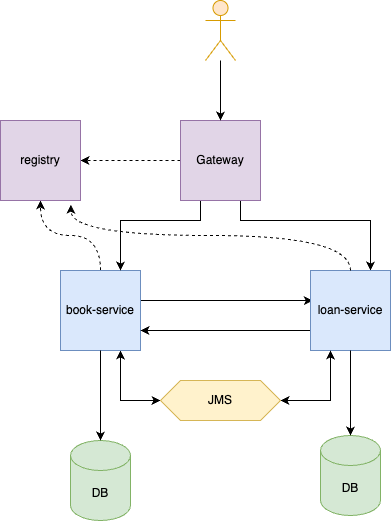
\includegraphics[width=0.5\textwidth]{img/neolib.png}
    \caption{Architecture générale du système}
    \label{fig:architecture}
\end{figure}

\subsection{book-service}

Ce service est une simple base de données de livres. L'API permet de lister les livres,
d'en ajouter, d'en supprimer et de les modifier. Les champs suivants sont disponibles pour
chaque livre:

\begin{itemize}
    \item ID (généré automatiquement)
    \item ISBN
    \item Titre
    \item Auteur
    \item Statut
\end{itemize}

Le statut permet de savoir si le livre est disponible, emprunté, perdu ou bloqué. 


\subsection{loan-service}

Ce service permet la gestion des emprunts ainsi que des utilisateurs. 
Un utilisateur doit exister dans la base de données pour pouvoir emprunter un livre. 

L'API permet d'emprunter un livre, de le rendre, de lister les emprunts en cours (pour un utilisateur donné)
et de savoir qui a emprunté un livre donné. De plus, il est possible de marquer un livre comme perdu. 


\section{Flux de communications entre les services}

\subsection{Flux de communication synchrones}

Les flux de communication synchrones sont effectués en utilisant le protocole HTTP. Ils sont 
uniquement utilisés pour effectuer des requêtes depuis le service \textit{loan-service} vers le service
\textit{book-service}. 

Il y a deux cas d'utilisation des communications synchrones:

\begin{itemize}
  \item Lors de l'emprunt d'un livre, le service \textit{loan-service} doit récupérer 
    les informations du livre (méta-données) pour compléter sa base de données locale et pour 
    vérifier que le livre est bien disponible ; 

  \item Lors de la perte d'un livre, le service \textit{loan-service} doit marquer le livre
    comme perdu dans la base de données du service \textit{book-service}.
\end{itemize}

Afin d'effectuer du \textit{client-side load balancing}, on utilise un client Feign pour effectuer
les requêtes HTTP.

\subsection{Flux de communication asynchrones}

Les flux de communication asynchrones sont effectués en utilisant le protocole AMQP. Ils sont
utilisés pour la communications entres les services, dans les deux sens. Ils permettent 
de notifier sans attendre de réponse. 

Ils sont utilisés dans les cas suivants : 

\begin{itemize}
  \item Lors de l'emprunt d'un livre, le service \textit{loan-service} doit notifier le service
    \textit{book-service} que le livre a été emprunté, pour la mise à jour du statut du livre ; 
    
  \item Lors du retour d'un livre, le service \textit{loan-service} doit notifier le service
    \textit{book-service} que le livre a été rendu, pour la mise à jour du statut du livre ; 

  \item Lorsque les méta-données d'un livre sont modifiées, le service \textit{book-service} doit
    notifier le service \textit{loan-service} pour la mise à jour des informations dans la base de données
    du service \textit{loan-service}.
\end{itemize}



\section{Guide de démarrage}

Dans cette section, on décrit la procédure qui permet de démarrer correctement les services. 

\subsection{Prérequis}

Il est nécessaire d'avoir installé les logiciels suivants:

\begin{itemize}
  \item Java 17
  \item Maven 3.9
  \item Docker 25
  \item Docker Compose 2.24
\end{itemize}

\subsection{Démarrage des services}

Tout d'abord, lancer le Docker Compose pour démarrer RabbitMQ et les bases de données mySQL : 

\begin{lstlisting}[language=bash]
docker-compose up -d
\end{lstlisting}

Ensuite, lancer les services un par un (si possible dans des terminaux séparés). Pour 
le service \textit{book-service}, on lance 3 instances et pour le service \textit{loan-service},
on lance 2 instances. Ceci permet de tester le \textit{load balancing}.

\begin{lstlisting}[language=bash]
  cd registry-service
  mvn spring-boot:run
\end{lstlisting}

\begin{lstlisting}[language=bash]
  cd api-gateway
  mvn spring-boot:run
\end{lstlisting}

\begin{lstlisting}[language=bash]
  cd book-service
  mvn spring-boot:run -Dspring-boot.run.arguments=--server.port=9901
  mvn spring-boot:run -Dspring-boot.run.arguments=--server.port=9902
  mvn spring-boot:run -Dspring-boot.run.arguments=--server.port=9903
\end{lstlisting}

\begin{lstlisting}[language=bash]
  cd loan-service
  mvn spring-boot:run -Dspring-boot.run.arguments=--server.port=9801
  mvn spring-boot:run -Dspring-boot.run.arguments=--server.port=9802
\end{lstlisting}

Alternativement, on peut lancer les services avec IntelliJ IDEA, qui permet 
de lancer les services en parallèle de manière plus simple. 

Pour tester les différents services, il est possible d'utiliser Postman. Un fichier 
\textit{postman.json} est fourni à la racine du projet, qui contient la configuration 
nécessaire pour tester les services. 

\section{Conclusion}

Ce projet a permis de mettre en pratique les concepts du pattern \textit{microservices} que nous avons
étudié en cours. 
L'application en tant que telle n'a en réalité pas beaucoup de sens et n'a pas de nécessité d'utiliser 
ce pattern. Il a fallu inventer des cas d'utilisation pour remplir les contraintes du projet, ce qui 
donne une implémentation qui manque parfois de sens. 

Dans l'ensemble, les concepts ont bien été mis en pratique et les services communiquent correctement 
entre eux. Le load balancing fonctionne correctement et les services sont bien enregistrés auprès du
registre Eureka. 

D'autres améliorations pourraient être apportées, comme par exemple la gestion de l'authentification, 
la possibilité de gérer les utilisateurs, de gérer les retards et les amendes, de prolonger un emprunt, 
ou encore d'effectuer une réservation de livre. 
 
\end{document}
